\documentclass[10pt]{beamer}
\usetheme{Madrid}
\usecolortheme{default}

\usepackage{amsmath,amssymb,amsfonts}
\usepackage{algorithm}
\usepackage{algorithmic}
\usepackage{graphicx}
\usepackage{tikz}
\usepackage{booktabs}
\usepackage{xcolor}

\title{Unpaired Neural Schrödinger Bridge (UNSB)}
\subtitle{Adversarial Learning for Unpaired Image-to-Image Translation}
\author{Research Presentation}
\date{\today}

\begin{document}

\frame{\titlepage}

\begin{frame}{Outline}
\tableofcontents
\end{frame}

\section{Motivation and Background}

\begin{frame}{The Core Problem}
\begin{block}{Central Challenge}
Learn a \alert{stochastic mapping} between two distributions $\pi_0$ and $\pi_1$ without paired data
\end{block}

\begin{columns}
\begin{column}{0.5\textwidth}
\textbf{Limitations of existing methods:}
\begin{itemize}
    \item CycleGAN: Requires cycle-consistency
    \item Diffusion models: High training cost
    \item Optimal Transport: Deterministic, lacks diversity
\end{itemize}
\end{column}

\begin{column}{0.5\textwidth}
\textbf{UNSB advantages:}
\begin{itemize}
    \item \textcolor{blue}{No paired data needed}
    \item \textcolor{blue}{Stochastic mapping}
    \item \textcolor{blue}{Theoretical guarantees}
    \item \textcolor{blue}{Efficient training}
\end{itemize}
\end{column}
\end{columns}
\end{frame}

\begin{frame}{What is Schrödinger Bridge?}
\begin{block}{Definition}
The Schrödinger Bridge (SB) seeks the \alert{optimal stochastic process} connecting two distributions that minimizes:
\begin{equation}
\min_{p(x_t)} \text{KL}(p(x_t) \| q(x_t))
\end{equation}
where $q(x_t)$ is a reference process (typically Ornstein-Uhlenbeck)
\end{block}

\begin{alertblock}{Key Properties}
\begin{itemize}
    \item SB is a \textbf{dynamic process}: $x_0 \sim \pi_0 \rightarrow x_t \rightarrow x_1 \sim \pi_1$
    \item Compared to OT, SB provides \textbf{stochasticity} and \textbf{smooth paths}
    \item Traditional SB requires \textcolor{red}{expensive iterative solving} (Sinkhorn iterations)
\end{itemize}
\end{alertblock}

\pause
\vspace{0.3cm}
\textbf{Question:} Why is stochasticity important in image translation?
\end{frame}

\section{Core Innovation: Markov Decomposition}

\begin{frame}{The Key Insight}
\begin{block}{Main Theorem}
UNSB represents SB as a composition of generators learned via \alert{adversarial learning}
\end{block}

\textbf{Time discretization:} Given partition $\{t_i\}_{i=0}^N$ of $[0,1]$ where $t_0=0, t_N=1$

\begin{equation}
p(\{x_{t_n}\}) = \textcolor{blue}{p(x_{t_N}|x_{t_{N-1}})} \textcolor{green!50!black}{p(x_{t_{N-1}}|x_{t_{N-2}})} \cdots \textcolor{orange}{p(x_{t_1}|x_{t_0})} p(x_{t_0})
\end{equation}

\begin{center}
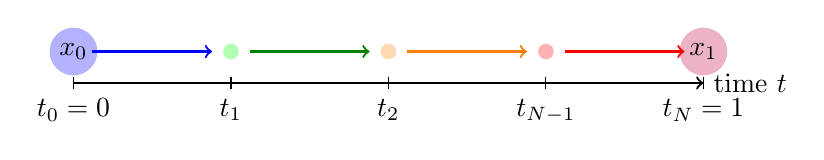
\begin{tikzpicture}[scale=0.8]
\draw[->, thick] (0,0) -- (10,0) node[right] {time $t$};
\foreach \x/\label in {0/$t_0=0$, 2.5/$t_1$, 5/$t_2$, 7.5/$t_{N-1}$, 10/$t_N=1$}
    \draw (\x,0.1) -- (\x,-0.1) node[below] {\label};
\node[circle, fill=blue!30, inner sep=2pt] at (0,0.5) {$x_0$};
\node[circle, fill=green!30, inner sep=2pt] at (2.5,0.5) {};
\node[circle, fill=orange!30, inner sep=2pt] at (5,0.5) {};
\node[circle, fill=red!30, inner sep=2pt] at (7.5,0.5) {};
\node[circle, fill=purple!30, inner sep=2pt] at (10,0.5) {$x_1$};
\draw[->, thick, blue] (0.3,0.5) -- (2.2,0.5);
\draw[->, thick, green!50!black] (2.8,0.5) -- (4.7,0.5);
\draw[->, thick, orange] (5.3,0.5) -- (7.2,0.5);
\draw[->, thick, red] (7.8,0.5) -- (9.7,0.5);
\end{tikzpicture}
\end{center}

\textbf{Inductive strategy:} Learn $p(x_{t_{i+1}}|x_{t_i})$ assuming we can sample from $p(x_{t_i})$
\end{frame}

\begin{frame}{Why Time Decomposition?}
\pause
\textbf{Challenge 1: Infinite-dimensional complexity}
\begin{itemize}
    \item Entire trajectory $\{x_t\}_{t\in[0,1]}$ is an infinite-dimensional object
    \item Direct learning: intractable path-space distribution
    \item Decomposition: learn simple conditional distributions
\end{itemize}

\pause
\vspace{0.3cm}
\textbf{Challenge 2: No intermediate data}
\begin{itemize}
    \item Only have marginals $\pi_0$ and $\pi_1$
    \item No access to trajectory samples
    \item Path density is incomputable
\end{itemize}

\pause
\vspace{0.3cm}
\textbf{Solution:} Learn $p(x_1|x_{t_i})$ (endpoint prediction) using adversarial matching against $\pi_1$

\pause
\vspace{0.3cm}
\textbf{Question:} How can we recover $p(x_{t_{i+1}}|x_{t_i})$ from $p(x_1|x_{t_i})$?
\end{frame}

\begin{frame}{Conditional Generator Design}
\begin{block}{Generator Definition}
For each time step $t_i$, define parameterized conditional distribution:
\begin{equation}
q_{\phi_i}(x_1|x_{t_i}) \quad \text{(DNN predicting target domain image)}
\end{equation}
\end{block}

\begin{columns}
\begin{column}{0.5\textwidth}
\textbf{Induced distributions:}
\begin{align}
q_{\phi_i}(x_{t_i}, x_1) &:= q_{\phi_i}(x_1|x_{t_i})p(x_{t_i}) \\
q_{\phi_i}(x_1) &:= \mathbb{E}_{p(x_{t_i})}[q_{\phi_i}(x_1|x_{t_i})]
\end{align}
\end{column}

\begin{column}{0.5\textwidth}
\begin{center}
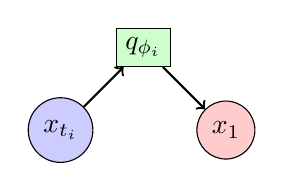
\begin{tikzpicture}[scale=0.7]
\node[draw, circle, fill=blue!20] (xti) at (0,0) {$x_{t_i}$};
\node[draw, circle, fill=red!20] (x1) at (3,0) {$x_1$};
\node[draw, rectangle, fill=green!20] (gen) at (1.5,1.5) {$q_{\phi_i}$};
\draw[->, thick] (xti) -- (gen);
\draw[->, thick] (gen) -- (x1);
\end{tikzpicture}
\end{center}
\end{column}
\end{columns}

\vspace{0.3cm}
\begin{alertblock}{Objective}
Optimize $\phi_i$ such that $q_{\phi_i}(x_1|x_{t_i}) = p(x_1|x_{t_i})$
\end{alertblock}
\end{frame}

\section{Theorem 1: Optimization Objective}

\begin{frame}{Theorem 1: Constrained Optimization}
\begin{theorem}[Core UNSB Theorem]
For any $t_i$, consider the following constrained optimization:
\begin{align}
\min_{\phi_i} \quad & \mathcal{L}_{\text{SB}}(\phi_i, t_i) := \mathbb{E}_{q_{\phi_i}(x_{t_i}, x_1)}[\|x_{t_i} - x_1\|^2] \notag \\
& \quad - 2\tau(1-t_i)\textcolor{blue}{H(q_{\phi_i}(x_{t_i}, x_1))} \tag{9} \\
\text{s.t.} \quad & \mathcal{L}_{\text{Adv}}(\phi_i, t_i) := D_{\text{KL}}(q_{\phi_i}(x_1) \| p(x_1)) = 0 \tag{10}
\end{align}
\end{theorem}

\begin{block}{Two Key Components}
\begin{enumerate}
    \item \textbf{SB Loss} $\mathcal{L}_{\text{SB}}$: Transport cost + entropy regularization
    \item \textbf{Adversarial Constraint} $\mathcal{L}_{\text{Adv}}$: Ensures marginal matching
\end{enumerate}
\end{block}
\end{frame}

\begin{frame}{Understanding the SB Loss}
\begin{equation}
\mathcal{L}_{\text{SB}}(\phi_i, t_i) = \underbrace{\mathbb{E}[\|x_{t_i} - x_1\|^2]}_{\text{Transport Cost}} - \underbrace{2\tau(1-t_i)H(q_{\phi_i}(x_{t_i}, x_1))}_{\text{Entropy Regularization}}
\end{equation}

\begin{columns}
\begin{column}{0.5\textwidth}
\textbf{Transport cost:}
\begin{itemize}
    \item Encourages $x_{t_i}$ close to $x_1$
    \item Minimizes expected squared distance
    \item Similar to Optimal Transport
\end{itemize}
\end{column}

\begin{column}{0.5\textwidth}
\textbf{Entropy regularization:}
\begin{itemize}
    \item \textcolor{blue}{$H(\cdot)$}: Joint entropy
    \item \textcolor{blue}{$\tau$}: Temperature parameter
    \item \textcolor{blue}{$(1-t_i)$}: Time weight
    \item Encourages \alert{diversity}
\end{itemize}
\end{column}
\end{columns}

\vspace{0.3cm}
\begin{alertblock}{Trade-off}
$\tau \uparrow$ $\Rightarrow$ More stochastic mapping \quad | \quad $\tau \downarrow$ $\Rightarrow$ More deterministic
\end{alertblock}

\pause
\vspace{0.3cm}
\textbf{Question:} What happens if we remove entropy regularization ($\tau = 0$)?
\end{frame}

\begin{frame}{Why Entropy Regularization?}
\begin{block}{Without Entropy ($\tau = 0$)}
\begin{equation}
\min \mathbb{E}[\|x_{t_i} - x_1\|^2] \quad \Rightarrow \quad \text{Deterministic Optimal Transport}
\end{equation}
Result: Each $x_0$ maps to a unique $x_1$ (mode collapse)
\end{block}

\pause
\begin{block}{With Entropy ($\tau > 0$)}
\begin{equation}
\min \mathbb{E}[\|x_{t_i} - x_1\|^2] - \tau H(q) \quad \Rightarrow \quad \text{Stochastic Bridge}
\end{equation}
Result: Each $x_0$ maps to a distribution $p(x_1|x_0)$
\end{block}

\pause
\vspace{0.3cm}
\textbf{Time-dependent weight:} $(1-t_i)$
\begin{itemize}
    \item \textbf{Early stage} ($t_i$ small): High entropy $\Rightarrow$ exploration
    \item \textbf{Late stage} ($t_i \rightarrow 1$): Low entropy $\Rightarrow$ convergence
\end{itemize}

\pause
\vspace{0.3cm}
\textbf{Analogy:} Similar to annealing - high temperature (early) for exploration, low temperature (late) for refinement
\end{frame}

\begin{frame}{Computing Entropy in High Dimensions}
\textbf{Problem:} For 256×256 images, direct entropy computation is intractable!

\pause
\begin{block}{Solution: Energy-Based Model Approximation}
Define energy network $E_\psi(x_{t_i}, x_1)$ such that:
\begin{equation}
q(x_{t_i}, x_1) = \frac{\exp(-E_\psi(x_{t_i}, x_1))}{Z_\psi}
\end{equation}

Then entropy can be approximated:
\begin{equation}
H(q) \approx \mathbb{E}_q[E_\psi(x_{t_i}, x_1)] + \log Z_\psi
\end{equation}
\end{block}

\pause
\textbf{Training strategy:}
\begin{itemize}
    \item \textcolor{blue}{Positive pairs}: $(x_{t_i}, x_1)$ from same trajectory $\rightarrow$ high energy
    \item \textcolor{red}{Negative pairs}: $(x_{t_i}, x_1')$ from different trajectories $\rightarrow$ low energy
    \item Use \texttt{logsumexp} for numerically stable $\log Z_\psi$ approximation
\end{itemize}

\pause
\vspace{0.3cm}
\textbf{Question:} How does this contrastive approach help estimate entropy?
\end{frame}

\begin{frame}{The Adversarial Constraint}
\begin{equation}
\mathcal{L}_{\text{Adv}}(\phi_i, t_i) := D_{\text{KL}}(q_{\phi_i}(x_1) \| p(x_1)) = 0
\end{equation}

\begin{block}{Meaning}
The marginal distribution $q_{\phi_i}(x_1)$ must match the true target distribution $p(x_1)$
\end{block}

\pause
\textbf{Why KL = 0 (exact matching)?}
\begin{itemize}
    \item Strong constraint: requires \alert{perfect distribution match}
    \item In practice: approximated via GAN training
    \item Theorem 1 proof requires exact marginal matching
\end{itemize}

\pause
\vspace{0.3cm}
\begin{columns}
\begin{column}{0.5\textwidth}
\textbf{Generator objective:}
\begin{itemize}
    \item Minimize $\mathcal{L}_{\text{SB}}$
    \item Fool discriminator
\end{itemize}
\end{column}

\begin{column}{0.5\textwidth}
\textbf{Discriminator objective:}
\begin{itemize}
    \item Distinguish $q_{\phi_i}(x_1)$ from $p(x_1)$
    \item Enforce marginal constraint
\end{itemize}
\end{column}
\end{columns}

\pause
\vspace{0.3cm}
\textbf{Question:} Can we relax this to $D_{\text{KL}} \approx 0$ in practice?
\end{frame}

\begin{frame}{Gaussian Transition Kernel}
\textbf{Key insight:} SB optimal process is closest to Brownian motion

Define transition distribution:
\begin{equation}
p(x_{t_{i+1}}|x_{t_i}, x_1) := \mathcal{N}\left(x_{t_{i+1}}\mid s_{i+1}x_1 + (1-s_{i+1})x_{t_i}, \textcolor{blue}{s_{i+1}(1-s_{i+1})\tau(1-t_i)}I\right)
\end{equation}
where $s_{i+1} := \frac{t_{i+1} - t_i}{1 - t_i}$

\pause
\begin{block}{Induced Conditional Distribution}
\begin{equation}
q_{\phi_i}(x_{t_{i+1}}|x_{t_i}) := \mathbb{E}_{q_{\phi_i}(x_1|x_{t_i})}[p(x_{t_{i+1}}|x_{t_i}, x_1)]
\end{equation}
\end{block}

\pause
\textbf{Understanding the distribution:}
\begin{itemize}
    \item \textbf{Mean}: $s_{i+1}x_1 + (1-s_{i+1})x_{t_i}$ interpolates between current and endpoint
    \item \textbf{Variance}: $s_{i+1}(1-s_{i+1})\tau(1-t_i)$ varies with time
    \item This is discretization of Ornstein-Uhlenbeck process
\end{itemize}

\pause
\vspace{0.3cm}
\textbf{Question:} Why take expectation over $x_1$ instead of using a fixed endpoint?
\end{frame}

\begin{frame}{Theorem 1 Conclusion}
\begin{theorem}[Continued]
If $\phi_i$ solves the optimization problem (Eq. 9-10), then:
\begin{equation}
\boxed{
\begin{aligned}
q_{\phi_i}(x_1|x_{t_i}) &= p(x_1|x_{t_i}) \\
q_{\phi_i}(x_{t_{i+1}}|x_{t_i}) &= p(x_{t_{i+1}}|x_{t_i}) \\
q_{\phi_i}(x_{t_{i+1}}) &= p(x_{t_{i+1}})
\end{aligned}
}
\end{equation}
\end{theorem}

\pause
\begin{alertblock}{Power of the Theorem}
\begin{enumerate}
    \item Learned generator $q_{\phi_i}$ exactly recovers true SB posterior $p(x_1|x_{t_i})$
    \item Induced next-step distribution $q_{\phi_i}(x_{t_{i+1}}|x_{t_i})$ is also correct
    \item Marginal distribution $q_{\phi_i}(x_{t_{i+1}})$ matches true distribution
\end{enumerate}
\end{alertblock}

\pause
\vspace{0.2cm}
\textcolor{blue}{\textbf{Recursive application}}: With $p(x_{t_{i+1}})$, we can learn $p(x_{t_{i+2}}|x_{t_{i+1}})$, and so on!

\pause
\vspace{0.3cm}
\textbf{Key insight:} Learn endpoint prediction $\Rightarrow$ automatically get entire Markov chain
\end{frame}

\section{Algorithm and Implementation}

\begin{frame}{Training Algorithm Overview}
\begin{algorithm}[H]
\small
\caption{UNSB Training}
\begin{algorithmic}[1]
\FOR{each training iteration}
    \STATE Sample $x_0 \sim \pi_0$ (source), $x_1 \sim \pi_1$ (target)
    \STATE Randomly select time step $t \in \{0, 1, \ldots, T-1\}$
    \STATE \textcolor{blue}{// Forward simulation (with gradient detachment)}
    \FOR{$i = 0$ to $t$}
        \STATE $X_{t_i} \leftarrow$ OU process update (detach)
        \STATE $\hat{X}_{t_i} \leftarrow G(X_{t_i}, t_i, z)$ (detach)
    \ENDFOR
    \STATE \textcolor{blue}{// Update discriminator}
    \STATE $\mathcal{L}_D \leftarrow$ LSGAN loss
    \STATE Update discriminator parameters
    \STATE \textcolor{blue}{// Update energy network}
    \STATE $\mathcal{L}_E \leftarrow$ Contrastive energy loss
    \STATE Update energy network parameters
    \STATE \textcolor{blue}{// Update generator}
    \STATE $\mathcal{L}_G \leftarrow \lambda_{\text{GAN}}\mathcal{L}_{\text{GAN}} + \lambda_{\text{SB}}\mathcal{L}_{\text{SB}} + \lambda_{\text{NCE}}\mathcal{L}_{\text{NCE}}$
    \STATE Update generator parameters
\ENDFOR
\end{algorithmic}
\end{algorithm}
\end{frame}

\begin{frame}{Time Scheduling Strategy}
\textbf{Non-uniform time grid:}
\begin{equation}
\text{increments} = \left[0, 1, \frac{1}{2}, \frac{1}{3}, \ldots, \frac{1}{T-1}\right]
\end{equation}
Cumulative sum and normalize: emphasizes later time steps

\begin{center}
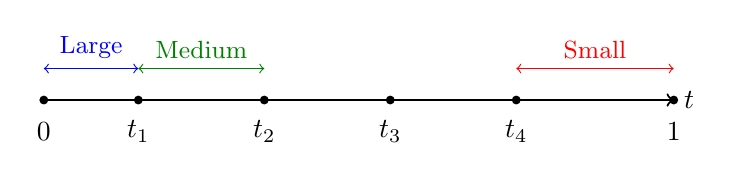
\begin{tikzpicture}[scale=0.8]
\draw[->, thick] (0,0) -- (10,0) node[right] {$t$};
\foreach \x in {0, 1.5, 3.5, 5.5, 7.5, 10}
    \fill (\x,0) circle (2pt);
\node at (0,-0.5) {$0$};
\node at (1.5,-0.5) {$t_1$};
\node at (3.5,-0.5) {$t_2$};
\node at (5.5,-0.5) {$t_3$};
\node at (7.5,-0.5) {$t_4$};
\node at (10,-0.5) {$1$};
\draw[<->, blue] (0,0.5) -- (1.5,0.5) node[midway, above] {\small Large};
\draw[<->, green!50!black] (1.5,0.5) -- (3.5,0.5) node[midway, above] {\small Medium};
\draw[<->, red] (7.5,0.5) -- (10,0.5) node[midway, above] {\small Small};
\end{tikzpicture}
\end{center}

\pause
\textbf{Rationale:}
\begin{itemize}
    \item \textbf{Early stage}: Large steps for rapid approach to target distribution
    \item \textbf{Late stage}: Small steps for fine-grained refinement
    \item Matches OU process characteristics
    \item Synergizes with time-decaying entropy weight $(1-t_i)$
\end{itemize}

\pause
\vspace{0.3cm}
\textbf{Question:} Why not use uniform spacing $t_i = i/T$?
\end{frame}

\begin{frame}{UNSB vs. Diffusion Models}
\begin{columns}
\begin{column}{0.5\textwidth}
\textbf{Diffusion Models:}
\begin{itemize}
    \item Fixed forward process (noise)
    \item Learn reverse denoising
    \item Requires many time steps (1000+)
    \item Slow training and inference
    \item Usually need paired data
\end{itemize}
\end{column}

\begin{column}{0.5\textwidth}
\textbf{UNSB:}
\begin{itemize}
    \item Learned forward process
    \item Directly predict target $x_1$
    \item Few time steps (5)
    \item Fast training and inference
    \item \textcolor{blue}{No paired data}
\end{itemize}
\end{column}
\end{columns}

\pause
\vspace{0.3cm}
\textbf{Key differences:}
\begin{itemize}
    \item UNSB is \alert{bidirectional} (learns bridge $\pi_0 \rightarrow \pi_1$)
    \item Diffusion is unidirectional (noise $\rightarrow$ data)
    \item UNSB has theoretical optimality guarantees (Schrödinger Bridge)
\end{itemize}

\pause
\vspace{0.3cm}
\textbf{Question:} What enables UNSB to use so few time steps compared to diffusion?
\end{frame}

\begin{frame}{UNSB vs. CycleGAN}
\begin{columns}
\begin{column}{0.5\textwidth}
\textbf{CycleGAN:}
\begin{itemize}
    \item Cycle consistency: $F(G(x)) \approx x$
    \item \textcolor{red}{Assumption}: Mapping invertible
    \item Deterministic mapping
    \item May produce artifacts
    \item No theoretical optimality
\end{itemize}
\end{column}

\begin{column}{0.5\textwidth}
\textbf{UNSB:}
\begin{itemize}
    \item SB optimality
    \item \textcolor{blue}{No invertibility required}
    \item Stochastic mapping (more realistic)
    \item Smoother transitions
    \item Theoretical guarantees
\end{itemize}
\end{column}
\end{columns}

\pause
\vspace{0.3cm}
\textbf{Experimental comparison (MRI):}
\begin{itemize}
    \item UNSB SSIM: 0.82 vs CycleGAN: 0.78
    \item UNSB preserves more anatomical details
    \item UNSB generates more natural textures
\end{itemize}

\pause
\vspace{0.3cm}
\textbf{Question:} When would cycle consistency assumption be violated in practice?
\end{frame}

\section{Limited Paired Data: Hybrid Training}

\begin{frame}{When Limited Paired Data is Available}
\textbf{Scenario:} Most data is unpaired, but small amount of paired data exists

\pause
\begin{block}{Scheme A: SB GT Transport}
Add ground truth guidance within SB framework:
\begin{equation}
\mathcal{L}_{\text{SB}} \rightarrow \mathcal{L}_{\text{SB}} + \tau\|\hat{X}_t - X_{\text{GT}}\|^2
\end{equation}
\end{block}

\pause
\textbf{Key advantages:}
\begin{itemize}
    \item Maintains SB mathematical structure
    \item Coefficient $\tau$ consistent with entropy regularization
    \item GT guidance naturally integrated as additional transport cost
    \item Doesn't break theoretical guarantees
\end{itemize}

\pause
\vspace{0.3cm}
\textbf{Two-stage training strategy:}
\begin{enumerate}
    \item \textbf{Stage 1 (Unpaired):} Learn from abundant unpaired data
    \begin{equation}
    \min \mathcal{L}_{\text{SB}} + \lambda_{\text{GAN}}\mathcal{L}_{\text{GAN}} + \lambda_{\text{NCE}}\mathcal{L}_{\text{NCE}}
    \end{equation}
    \item \textbf{Stage 2 (Paired fine-tuning):} Refine with limited paired data
    \begin{equation}
    \min \mathcal{L}_{\text{SB}} + \tau\|\hat{X}_t - X_{\text{GT}}\|^2 + \lambda_{\text{GAN}}\mathcal{L}_{\text{GAN}}
    \end{equation}
\end{enumerate}
\end{frame}

\begin{frame}{Unpaired + Paired Two-Stage Training}
\begin{center}
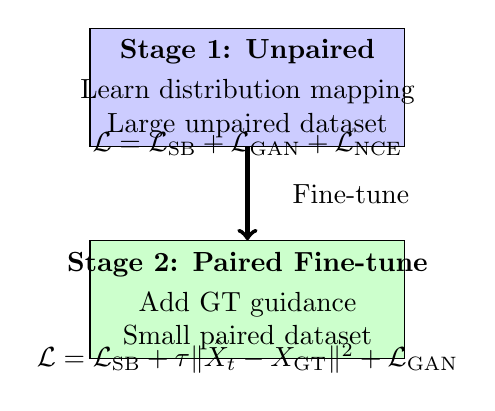
\begin{tikzpicture}[scale=0.9]
% Stage 1
\node[draw, rectangle, fill=blue!20, minimum width=4cm, minimum height=1.5cm] (stage1) at (0,2) {};
\node at (0,2.5) {\textbf{Stage 1: Unpaired}};
\node[align=center] at (0,1.7) {Learn distribution mapping\\Large unpaired dataset};
\node at (0,1.2) {$\mathcal{L} = \mathcal{L}_{\text{SB}} + \mathcal{L}_{\text{GAN}} + \mathcal{L}_{\text{NCE}}$};

% Stage 2
\node[draw, rectangle, fill=green!20, minimum width=4cm, minimum height=1.5cm] (stage2) at (0,-1) {};
\node at (0,-0.5) {\textbf{Stage 2: Paired Fine-tune}};
\node[align=center] at (0,-1.3) {Add GT guidance\\Small paired dataset};
\node at (0,-1.8) {$\mathcal{L} = \mathcal{L}_{\text{SB}} + \tau\|\hat{X}_t - X_{\text{GT}}\|^2 + \mathcal{L}_{\text{GAN}}$};

% Arrow
\draw[->, ultra thick] (stage1) -- (stage2);
\node[right] at (0.5,0.5) {Fine-tune};
\end{tikzpicture}
\end{center}

\pause
\textbf{Benefits:}
\begin{itemize}
    \item Stage 1: Captures general distribution structure (robust to overfitting)
    \item Stage 2: Adds precise pixel-level alignment (leverages paired supervision)
    \item Better than training from scratch with only paired data
\end{itemize}
\end{frame}

\section{Comparison with I2SB-Inversion}

\begin{frame}{I2SB-Inversion: Multicontrast MRI Reconstruction}
\textbf{Paper:} ``I2SB-Inversion: Multicontrast Guided Reconstruction via Schrödinger Bridge'' (arXiv:2411.14269)

\pause
\begin{block}{Core Framework}
\begin{itemize}
    \item Uses Schrödinger Bridge for \alert{guided reconstruction}
    \item Different contrasts (T1, T2, FLAIR) provide complementary information
    \item Incorporates multicontrast guidance during reverse process
\end{itemize}
\end{block}

\pause
\textbf{Key methodology:}
\begin{enumerate}
    \item \textbf{Forward process}: Add noise following Brownian motion
    \item \textbf{Reverse process}: Denoise guided by multicontrast observations
    \item \textbf{SB optimality}: Minimize expected cost between source and target
\end{enumerate}

\pause
\vspace{0.3cm}
\textbf{Two-stage training:}
\begin{itemize}
    \item \textbf{Stage 1}: Unconditional pretraining on distribution
    \item \textbf{Stage 2}: Guided fine-tuning with contrast conditioning
\end{itemize}
\end{frame}

\begin{frame}{UNSB vs. I2SB-Inversion: Key Differences}
\begin{table}
\small
\begin{tabular}{p{3cm}p{4cm}p{4cm}}
\toprule
\textbf{Aspect} & \textbf{UNSB} & \textbf{I2SB-Inversion} \\
\midrule
\textbf{Task} & Image-to-image translation & Image reconstruction \\
\midrule
\textbf{Data requirement} & \textcolor{blue}{Unpaired} (both domains) & Paired/unpaired multicontrast \\
\midrule
\textbf{Training stages} &
\begin{minipage}{3.5cm}
1. Unpaired distribution learning\\
2. Optional paired fine-tune
\end{minipage}
&
\begin{minipage}{3.5cm}
1. Unconditional pretraining\\
2. Multicontrast guidance
\end{minipage}
\\
\midrule
\textbf{Guidance} & Adversarial constraint on $\pi_1$ & Multicontrast observations \\
\midrule
\textbf{Key innovation} & No paired data needed & Leverages complementary contrasts \\
\bottomrule
\end{tabular}
\end{table}
\end{frame}

\begin{frame}{Deeper Comparison: Training Paradigms}
\begin{columns}
\begin{column}{0.5\textwidth}
\textbf{UNSB approach:}
\begin{enumerate}
    \item \textcolor{blue}{Unpaired stage}
    \begin{itemize}
        \item Learn $p(x_1|x_{t_i})$ via adversarial
        \item Only needs marginals $\pi_0$, $\pi_1$
        \item Entropy regularization for diversity
    \end{itemize}
    \item \textcolor{green!50!black}{Paired stage (optional)}
    \begin{itemize}
        \item Add GT transport cost
        \item Fine-tune within SB framework
    \end{itemize}
\end{enumerate}
\end{column}

\begin{column}{0.5\textwidth}
\textbf{I2SB-Inversion approach:}
\begin{enumerate}
    \item \textcolor{blue}{Unconditional stage}
    \begin{itemize}
        \item Learn data distribution
        \item Standard SB pretraining
        \item No guidance signals
    \end{itemize}
    \item \textcolor{green!50!black}{Guided stage}
    \begin{itemize}
        \item Condition on multiple contrasts
        \item Reconstruction constraints
        \item k-space consistency (MRI)
    \end{itemize}
\end{enumerate}
\end{column}
\end{columns}

\pause
\vspace{0.3cm}
\textbf{Similarity:} Both use two-stage training to separate distribution learning from task-specific refinement

\pause
\vspace{0.3cm}
\textbf{Difference:}
\begin{itemize}
    \item UNSB: Paired data is \alert{optional} enhancement
    \item I2SB-Inversion: Multicontrast guidance is \alert{essential} for task
\end{itemize}
\end{frame}

\begin{frame}{Paired Data Handling: Philosophical Difference}
\begin{alertblock}{UNSB Philosophy}
\textbf{Core capability}: Work entirely without paired data
\begin{itemize}
    \item Adversarial learning provides sufficient supervision
    \item Paired data ($\tau\|\hat{X}_t - X_{\text{GT}}\|^2$) is \textit{bonus} when available
    \item Two-stage: unpaired $\rightarrow$ optional paired fine-tune
\end{itemize}
\end{alertblock}

\pause
\begin{alertblock}{I2SB-Inversion Philosophy}
\textbf{Core capability}: Leverage multicontrast information
\begin{itemize}
    \item Guidance from multiple contrasts is central to method
    \item Can use paired or unpaired multicontrast data
    \item Two-stage: unconditional $\rightarrow$ contrast-guided reconstruction
\end{itemize}
\end{alertblock}

\pause
\vspace{0.3cm}
\textbf{Conceptual parallel:}
\begin{itemize}
    \item Both recognize value of \alert{separating} general distribution learning from specific supervision
    \item UNSB: Unpaired $\rightarrow$ Paired
    \item I2SB: Unconditional $\rightarrow$ Conditional
\end{itemize}
\end{frame}

\begin{frame}{Mathematical Formulation Comparison}
\textbf{UNSB optimization (per time step):}
\begin{equation}
\min_{\phi_i} \mathbb{E}[\|x_{t_i} - x_1\|^2] - 2\tau(1-t_i)H(q_{\phi_i}) + \textcolor{blue}{\tau\|\hat{x}_t - x_{\text{GT}}\|^2}
\end{equation}
\begin{equation}
\text{s.t. } D_{\text{KL}}(q_{\phi_i}(x_1) \| p(x_1)) = 0
\end{equation}

\pause
\vspace{0.5cm}
\textbf{I2SB-Inversion approach:}
\begin{itemize}
    \item Forward: $dx_t = f(x_t, t)dt + g(t)dW_t$
    \item Reverse: $dx_t = [f(x_t, t) - g^2(t)\nabla \log p_t(x_t|\mathbf{y})]dt + g(t)d\bar{W}_t$
    \item Guidance: $\nabla \log p_t(x_t|\mathbf{y})$ from multiple contrasts $\mathbf{y}$
\end{itemize}

\pause
\vspace{0.3cm}
\textbf{Key distinction:}
\begin{itemize}
    \item UNSB: GT term is additive cost in discrete Markov framework
    \item I2SB: Guidance enters through conditional score in continuous SDE
\end{itemize}
\end{frame}

\begin{frame}{When to Use Which Method?}
\begin{table}
\small
\begin{tabular}{p{4cm}p{3cm}p{3cm}}
\toprule
\textbf{Scenario} & \textbf{UNSB} & \textbf{I2SB-Inversion} \\
\midrule
No paired data, need domain translation & \textcolor{green!50!black}{\checkmark\checkmark} & \\
\midrule
Small amount paired data & \textcolor{green!50!black}{\checkmark} (fine-tune) & \\
\midrule
Multicontrast reconstruction & & \textcolor{green!50!black}{\checkmark\checkmark} \\
\midrule
Need few-step inference & \textcolor{green!50!black}{\checkmark\checkmark} (5 steps) & \textcolor{orange}{$\sim$} (depends) \\
\midrule
MRI with k-space & \textcolor{orange}{Adaptable} & \textcolor{green!50!black}{\checkmark\checkmark} (native) \\
\midrule
Natural image translation & \textcolor{green!50!black}{\checkmark\checkmark} & \textcolor{orange}{Overkill} \\
\bottomrule
\end{tabular}
\end{table}

\pause
\vspace{0.3cm}
\textbf{Summary:}
\begin{itemize}
    \item \textbf{UNSB}: General-purpose unpaired translation with optional paired enhancement
    \item \textbf{I2SB-Inversion}: Specialized reconstruction with multicontrast guidance
\end{itemize}
\end{frame}

\section{Theoretical Insights and Questions}

\begin{frame}{Q\&A: Why KL Divergence = 0?}
\textbf{Question:} The constraint $D_{\text{KL}}(q_{\phi_i}(x_1) \| p(x_1)) = 0$ seems too strong. Can we achieve this in practice?

\pause
\textbf{Answer:}
\begin{enumerate}
    \item \textbf{Theoretical requirement}
    \begin{itemize}
        \item Theorem 1 proof requires exact marginal matching
        \item Otherwise $q_{\phi_i}(x_1|x_{t_i}) \neq p(x_1|x_{t_i})$
        \item Ensures correctness of induced Markov chain
    \end{itemize}

    \pause
    \item \textbf{Practical approximation}
    \begin{itemize}
        \item GAN training approximates the constraint
        \item Discriminator enforces $q_{\phi_i}(x_1) \approx p(x_1)$
        \item LSGAN loss provides stable training
    \end{itemize}

    \pause
    \item \textbf{Lagrangian perspective}
    \begin{itemize}
        \item Constrained optimization $\rightarrow$ unconstrained with weight $\lambda_{\text{GAN}}$
        \item Ablations show $\lambda_{\text{GAN}} \geq 1.0$ sufficient
        \item Trade-off between constraint satisfaction and optimization stability
    \end{itemize}
\end{enumerate}
\end{frame}

\begin{frame}{Q\&A: Inference Randomness}
\textbf{Question:} How does inference work? Is output different every time?

\pause
\textbf{Answer:}

\textbf{Inference procedure:}
\begin{enumerate}
    \item Given input $x_0$
    \item For $t = 0, 1, \ldots, T-1$:
    \begin{itemize}
        \item Compute $\hat{x}_1 = G(x_t, t, z)$ where $z \sim \mathcal{N}(0, I)$
        \item Update $x_{t+1} = (1-\alpha)x_t + \alpha\hat{x}_1 + \sqrt{\text{scale} \cdot \tau}\epsilon$
    \end{itemize}
    \item Output $x_T$ as final result
\end{enumerate}

\pause
\textbf{Sources of randomness:}
\begin{itemize}
    \item Noise $z$ input to generator
    \item OU diffusion noise $\epsilon$
\end{itemize}

\pause
\textbf{Controlling randomness:}
\begin{itemize}
    \item Fixed seed $\Rightarrow$ deterministic output
    \item Lower $\tau$ $\Rightarrow$ less stochastic
    \item Can sample multiple times and select best
\end{itemize}
\end{frame}

\begin{frame}{Q\&A: Advantage of Few Time Steps}
\textbf{Question:} What enables UNSB to use only 5 time steps versus 1000+ for diffusion models?

\pause
\textbf{Answer:}

\begin{enumerate}
    \item \textbf{Direct endpoint prediction}
    \begin{itemize}
        \item Generator predicts $p(x_1|x_t)$ directly
        \item Not gradual denoising like diffusion
        \item Each step makes significant progress
    \end{itemize}

    \pause
    \item \textbf{Learned forward process}
    \begin{itemize}
        \item Forward transitions are optimized, not fixed
        \item Adapts to specific $\pi_0 \rightarrow \pi_1$ mapping
        \item More efficient than generic noise schedule
    \end{itemize}

    \pause
    \item \textbf{Non-uniform time scheduling}
    \begin{itemize}
        \item Harmonic schedule: large early steps, small late steps
        \item Exploits OU process properties
        \item Synergizes with time-decaying entropy
    \end{itemize}

    \pause
    \item \textbf{Strong supervision}
    \begin{itemize}
        \item Adversarial constraint directly on $\pi_1$
        \item Transport cost + entropy regularization
        \item No need for small Gaussian approximation errors
    \end{itemize}
\end{enumerate}
\end{frame}

\section{Summary}

\begin{frame}{Core Contributions}
\begin{enumerate}
    \item \textbf{Theoretical innovation}
    \begin{itemize}
        \item Decompose Schrödinger Bridge into learnable generator sequence
        \item Avoid expensive Sinkhorn iterations via adversarial learning
        \item Theorem 1 provides correctness guarantees
    \end{itemize}

    \item \textbf{Algorithmic innovation}
    \begin{itemize}
        \item Energy network for high-dimensional entropy estimation
        \item Time scheduling strategy (harmonic series)
        \item Scheme A for leveraging limited paired data
    \end{itemize}

    \item \textbf{Practical advantages}
    \begin{itemize}
        \item No paired data required (unpaired learning)
        \item Few time steps ($T=5$) for efficiency
        \item State-of-the-art performance on MRI translation
        \item Two-stage training: unpaired + optional paired fine-tuning
    \end{itemize}
\end{enumerate}
\end{frame}

\begin{frame}{Connections to I2SB-Inversion}
\textbf{Shared philosophy:}
\begin{itemize}
    \item Both leverage Schrödinger Bridge framework
    \item Two-stage training separates distribution learning from task-specific refinement
    \item Recognize value of combining unsupervised and supervised signals
\end{itemize}

\pause
\vspace{0.3cm}
\textbf{Complementary strengths:}
\begin{itemize}
    \item \textbf{UNSB}: Excel at unpaired domain translation
    \begin{itemize}
        \item Stage 1: Learn from unpaired data
        \item Stage 2: Optional paired fine-tuning with $\tau\|\hat{X}_t - X_{\text{GT}}\|^2$
    \end{itemize}
    \item \textbf{I2SB-Inversion}: Excel at multicontrast reconstruction
    \begin{itemize}
        \item Stage 1: Unconditional pretraining
        \item Stage 2: Multicontrast guidance conditioning
    \end{itemize}
\end{itemize}

\pause
\vspace{0.3cm}
\textbf{Future direction:} Combine unpaired learning with multicontrast guidance for robust few-shot medical image translation
\end{frame}

\begin{frame}{Limitations and Future Work}
\textbf{Current limitations:}
\begin{itemize}
    \item Energy network training stability (logsumexp numerical issues)
    \item Hyperparameter sensitivity ($\tau$, $\lambda_{\text{SB}}$)
    \item Memory consumption for high-resolution images
\end{itemize}

\pause
\vspace{0.5cm}
\textbf{Future directions:}
\begin{enumerate}
    \item \textbf{Theory}: More rigorous convergence analysis
    \item \textbf{Architecture}: Transformer-based generators
    \item \textbf{Applications}:
    \begin{itemize}
        \item 3D medical imaging (CT/MRI volumes)
        \item Video translation with temporal consistency
        \item Multimodal fusion
    \end{itemize}
    \item \textbf{Efficiency}: Distillation to single-step generator
    \item \textbf{Control}: Text-guided Schrödinger Bridge
    \item \textbf{Hybrid}: Combine UNSB unpaired learning with I2SB multicontrast guidance
\end{enumerate}
\end{frame}

\begin{frame}{References}
\small
\begin{thebibliography}{99}
\bibitem{unsb} Gushchin, N., et al. (2023).
\textit{Unpaired Neural Schrödinger Bridge}.
arXiv:2305.15086.

\bibitem{i2sb} Liu, G., et al. (2024).
\textit{I2SB-Inversion: Multicontrast Guided Reconstruction via Schrödinger Bridge}.
arXiv:2411.14269.

\bibitem{sb} Chen, Y., et al. (2022).
\textit{Likelihood Training of Schrödinger Bridge using Forward-Backward SDEs Theory}.
ICLR 2022.

\bibitem{ot} Peyré, G., \& Cuturi, M. (2019).
\textit{Computational Optimal Transport}.
Foundations and Trends in Machine Learning.

\bibitem{cyclegan} Zhu, J. Y., et al. (2017).
\textit{Unpaired Image-to-Image Translation using Cycle-Consistent Adversarial Networks}.
ICCV 2017.
\end{thebibliography}
\end{frame}

\begin{frame}[standout]
Thank You!\\
\vspace{1cm}
\Large Questions?
\end{frame}

\end{document}
